\begin{myConceptSteps}{To find the maximum and minimum given the graph of a relation\dots}
    \myStep{dots}{Draw dots on the highest and lowest points on the curve.}
    \myStep{coordinates}{Find the $y$ coordinates of those points.}
    \myStep{maximum}{The maximum is the $y$ coordinate of the highest point.}
    \myStep{minimum}{The minimum is the $y$ coordinate of the lowest point.}
\end{myConceptSteps}


\begin{myExample}{
    Find the maximum and minimum of this relation.
    (The curve keeps on going forever off the top of the grid.)
    \begin{center}
        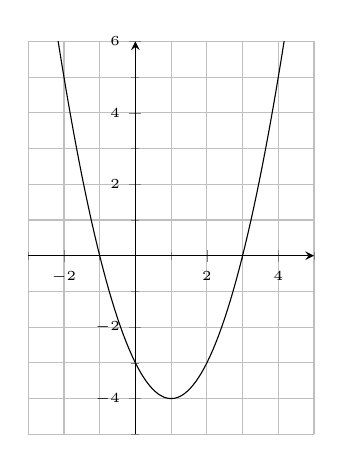
\begin{tikzpicture}
            \begin{axis}[
                width=3in,
                grid=both,
                axis x line = middle,axis y line = middle,
                axis equal image,
                xtick distance = 2, ytick distance = 2, 
                minor tick num = 1,
                xmin = -3, xmax=5,
                ymin = -5, ymax=6,
                tick label style = {font=\tiny},
                ]
                \addplot[no marks, samples=100, domain=-3:5, ] expression { (x-1)^2 - 4 };
            \end{axis}
        \end{tikzpicture}
    \end{center}
}
    \vspace{1.5in}
\end{myExample}

\begin{myExample}{
    Find the maximum and minimum of this relation.
    (The curve keeps on going forever off the bottom of the grid.)
    \begin{center}
        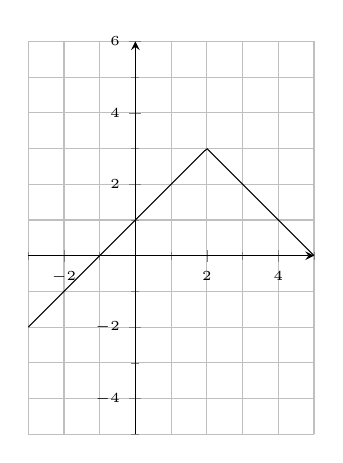
\begin{tikzpicture}
            \begin{axis}[
                width=3in,
                grid=both,
                axis x line = middle,axis y line = middle,
                axis equal image,
                xtick distance = 2, ytick distance = 2, 
                minor tick num = 1,
                xmin = -3, xmax=5,
                ymin = -5, ymax=6,
                tick label style = {font=\tiny},
                ]
                \addplot[no marks, samples=100, domain=-3:5, ] expression { -abs(x-2) +3 };
            \end{axis}
        \end{tikzpicture}
    \end{center}
}
    \vspace{1.5in}
\end{myExample}